\documentclass[a4paper]{article}
\usepackage[dutch]{babel}
\usepackage{amsthm,amsmath}
\usepackage{graphicx}
\usepackage{epstopdf}
\usepackage{enumerate}
\usepackage{amssymb}
\usepackage{float}
\usepackage{algpseudocode}
\usepackage{varwidth}
\usepackage{mcode}
\usepackage{algorithm}
\usepackage{caption}
\usepackage{subcaption}


\title{Numerieke Modellering en Benadering: Practicum 1}
\author{Jona Beysens \& Arnout Devos}

\newcommand{\opgave}[1]{\section*{Opgave #1}}
\newcommand{\dx}{\Delta x}
\newcommand{\dy}{\Delta y}
\newcommand{\dz}{\Delta z}
\newcommand{\dt}{\Delta t}

\begin{document}
\maketitle
\date
\opgave{1}
De nulpunten van een orthogonale veelterm gebaseerd op de waarden $\alpha_{k}$,$\beta_{k}$ en $\lambda_{k}$ kan gevonden worden door de eigenwaarden te bepalen een $n$ x $n$ tridiagonale matrix \textit{tridag($\nu_{k-1}$; $\alpha_{k}$; $\mu_{k-1}$)} met $\nu_{k} = \frac{\beta_{k+1}}{\lambda_{k+1}}$ en $\mu_{k} = \frac{1}{\lambda_{k}}$. Dit volgt uit \textbf{stelling 3.2.5 Numerieke Modellering en Benadering}.

De \textsc{Matlab}-code bevindt zich in bijlage 1.
\opgave{2}
Om de orthogonale veeltermen te evalueren kan effici\"ent gebruikt gemaakt worden van de drietermsrecursiebetrekking zoals gegeven in \textbf{stelling 3.2.3 Numerieke Modellering en Benadering}. Elk element uit de matrix $M$ wordt bepaald als volgt: $M_{ij} = \psi_{j}(x_{i})$. Aangezien in elke rij dezelfde $x_{i}$ ge\"evalueerd moet worden, maken we voor elke rij gebruik van de recursiebetrekking. De werking van de functie wordt getoond door in figuur \ref{fig:polynomials} de Chebyshev veeltermen $T_{1},T_{2},T_{3}$ en $T_{4}$ te evalueren in een voldoende aantal punten.

De \textsc{Matlab}-code bevindt zich in bijlage 2.
\begin{figure}
        \centering
        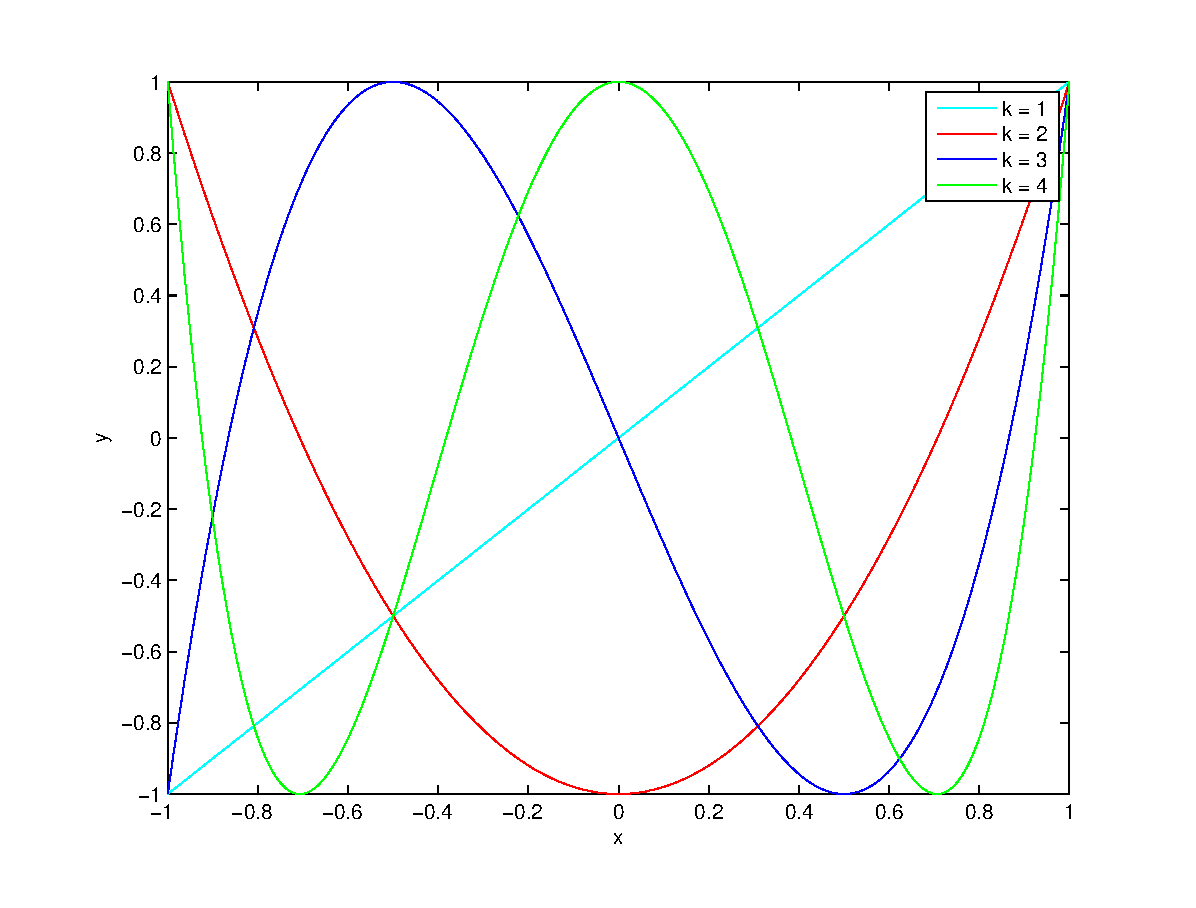
\includegraphics[width=\textwidth]{Jona/chebyshev_polynomials.eps}
        \caption{Chebyshev veeltermen $T_{1},T_{2},T_{3}$ en $T_{4}$ van respectievelijk graad $k=1,\dots,4$}
        \label{fig:polynomials}
    \end{figure}
\opgave{3}
De interpolerende veelterm $y_{n-1}$ voldoet aan volgende betrekking: $y_{n-1} = \sum\limits_{i=0}^{n-1}c_{i}T_{i}$. Om de co\"effici\"enten $c_{i}$ te vinden moet het stelsel $Mc = B$ met $M_{ij} = \psi_{j}(x_{i})$ en $B_{i} = f(x_{i})$ opgelost worden. Verder moet de veelterm ge\"evalueerd worden in een stel punten $t$. Dit wordt bekomen door het \textit{rekenschema van Smith} uit te werken dat het stel punten. Dit vermijdt de interpolerende veelterm te rangschikken naar opeenvolgende machten van $x$, d.w.z. de co\"effici\"enten $d_{i}$ te bepalen zodat $y_{n-1} = \sum\limits_{i=0}^{n-1}d_{i}x^{i}$ om daarna het \textit{rekenschema van Horner} toe te passen.

De \textsc{Matlab}-code bevindt zich in bijlage 3.
\opgave{4}
\begin{enumerate}[a)] % a), b), c), ...
\item
In figuur \ref{fig:lin_cos} en figuur \ref{fig:cheb_cos} wordt de functie $f_{1}(x) = cos(x)$ benaderd door middel van Chebyshev veeltermen. Zowel de interpolerende veeltermen  (\ref{fig:lin_cos_interpol} en \ref{fig:cheb_cos_interpol}) alsook de corresponderende fouten (\ref{fig:lin_cos_error} en \ref{fig:cheb_cos_error}) worden voorgesteld. 

In figuur \ref{fig:lin_cos} wordt gebruik gemaakt van equidistant verdeelde interpolatiepunten. Hierbij zien we dat de absolute fout afneemt naarmate de graad $n$ stijgt. Vanaf graad 3 valt de interpolerende veelterm bijna volledig samen met de te benaderen functie $f_{1}$. Verder zijn de interpolatiepunten duidelijk zichtbaar op figuur \ref{fig:lin_cos_error}. In de interpolatiepunten wordt de fout immers 0 en dus zakt de curve plots naar beneden.

In figuur \ref{fig:cheb_cos} wordt gebruik gemaakt van de nulpunten van de Chebyshev veelterm van graad $n+1$ als interpolatiepunten. Ook hier zakt de absolute fout bij stijgende graad $n$. Verder zijn de interpolatiepunten op te merken in figuur \ref{fig:cheb_cos_error}. Door het nemen van deze interpolatiepunten kan de fout verkleind worden. Dit is duidelijk te zien in de fout $e_{1}$ horende bij $y_{1}$. Bij equidistant verdeelde interpolatiepunten liggen deze voor graad 1 in de randpunten van het interval. Dit leidt tot een grote fout in het midden van het interval. Bij de nulpunten van Chebyshev veelterm van graad $n+1$ is dit niet het geval. De evolutie van de maximale fout in functie van graad $n$ wordt ook voorgesteld in figuur \ref{fig:error_global_cos}. Vanaf graad $n = 15$ neemt de fout bij equidistante interpolatie punten niet meer af.
\item
In figuur \ref{fig:lin_f2} en figuur \ref{fig:cheb_f2} wordt de functie $f_{2}(t) = \frac{1}{1+6x^{2}}$ benaderd door middel van Chebyshev veeltermen. Zowel de interpolerende veeltermen  (\ref{fig:lin_f2_interpol} en \ref{fig:cheb_f2_interpol}) alsook de corresponderende fouten (\ref{fig:lin_f2_error} en \ref{fig:cheb_f2_error}) worden voorgesteld. In dit geval worden Chebyshev veeltermen van graad $n=1,\dots,9$ gebruikt in plaats van $n=1,\dots,3$ aangezien deze functie $f_{2}$ moeilijker te benaderen is. In figuur \ref{fig:lin_f2_error} wordt de fout bij stijgende graad $n$ vanaf een bepaalde graad niet meer kleiner. Dit komt door het gebruik van equidistant verdeelde interpolatiepunten. Bij de nulpunten van Chebyshev veelterm van graad $n+1$ zakt de fout immers wel (zie figuur \ref{fig:cheb_f2_error}). 

De evolutie van de maximale fout in functie van graad $n$ wordt ook voorgesteld in figuur \ref{fig:error_global_f2}. Vanaf graad $n=5$ neemt de fout bij equidistante interpolatie punten niet meer af. Het is algemeen zo dat de fout bij hogere graad bij equidistante interpolatiepunten niet meer verkleint. Dit komt door sterke oscillatie tussen de interpolatiepunten aan de randen van het interval. Dit fenomeen is gekend als het \textit{Runge's phenomenon}.
\end{enumerate}


\begin{figure}
    \centering
    \begin{subfigure}[t]{0.45\textwidth}
        \centering
        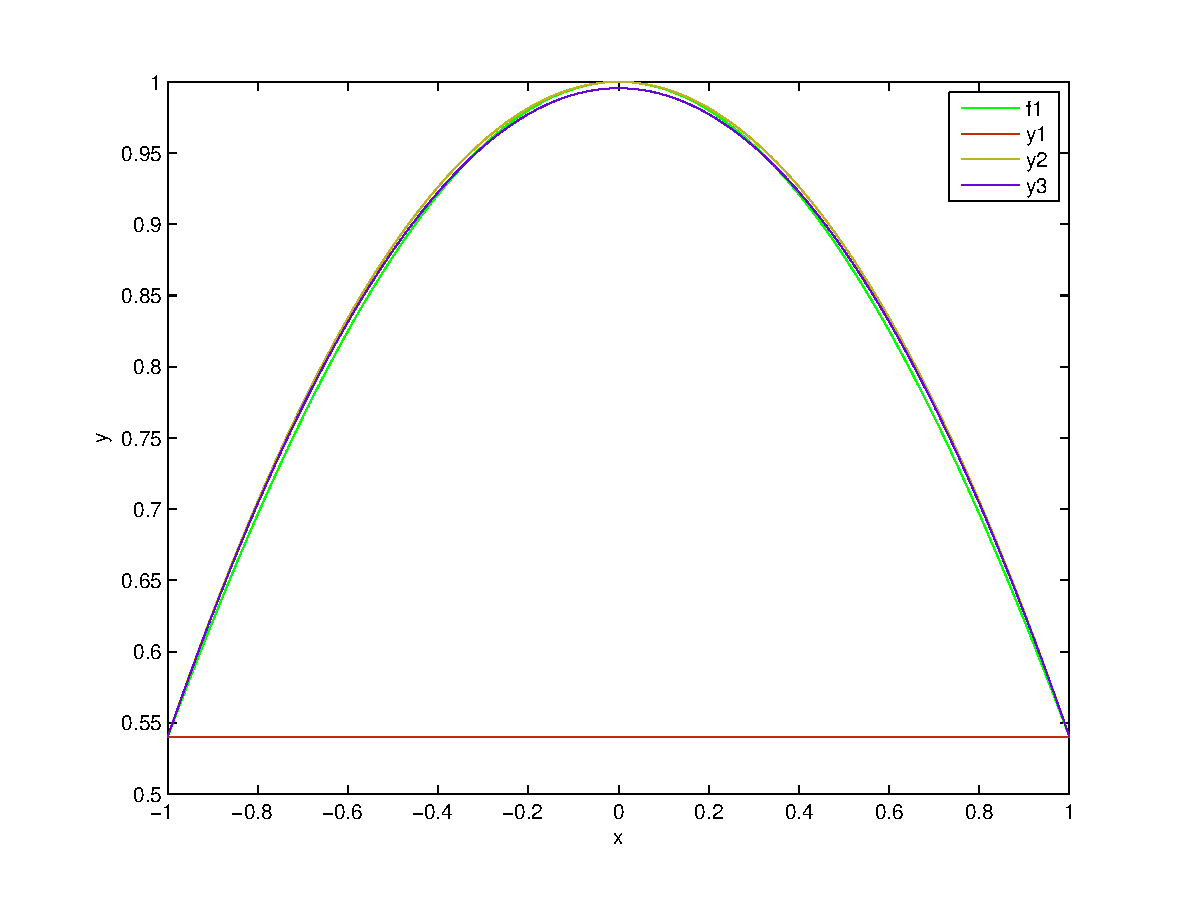
\includegraphics[width=\textwidth]{Jona/linspace_cos_interpolation.eps}
        \caption{Interpolerende Chebyshev veeltermen $y_{1},y_{2}$ en $y_{3}$ van respectievelijk graad $n=1,\dots,3$}
        \label{fig:lin_cos_interpol}
        \vspace*{1cm}
    \end{subfigure}
    \begin{subfigure}[t]{0.45\textwidth}
        \centering
        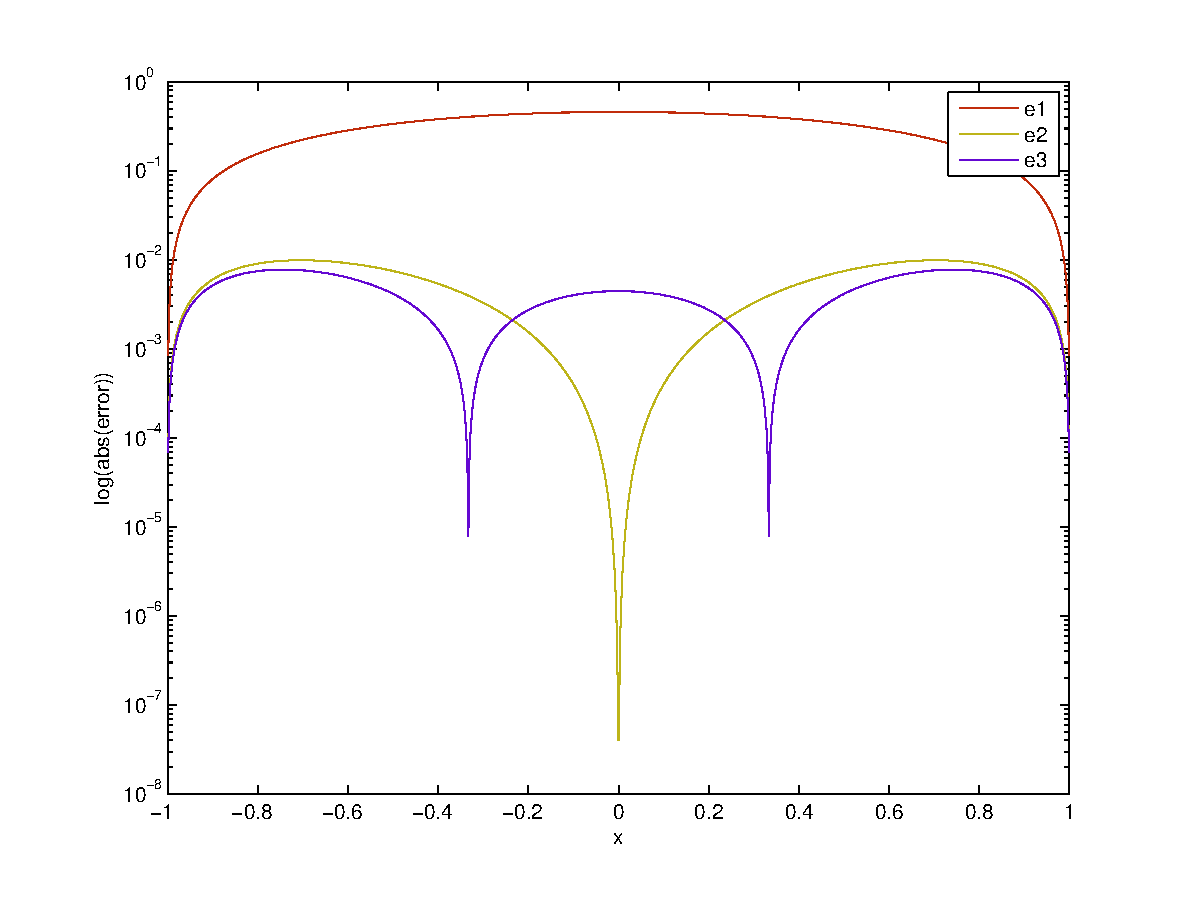
\includegraphics[width=\textwidth]{Jona/linspace_cos_error.eps}
        \caption{De fout $e_{n} = |y_{n}(t)-f(t)|$ van interpolerende Chebyshev veeltermen $y_{1},y_{2}$ en $y_{3}$ van respectievelijk graad $n=1,\dots,3$}
        \label{fig:lin_cos_error}
        %\vspace*{1cm}
    \end{subfigure}
    \hfill
    \caption{De functie $f_{1}(t) = cos(t)$ wordt benaderd in equidistant verdeelde interpolatiepunten door middel van Chebyshev veeltermen}\label{fig:lin_cos}.
\end{figure}

\begin{figure}
    \centering
    \begin{subfigure}[t]{0.45\textwidth}
        \centering
        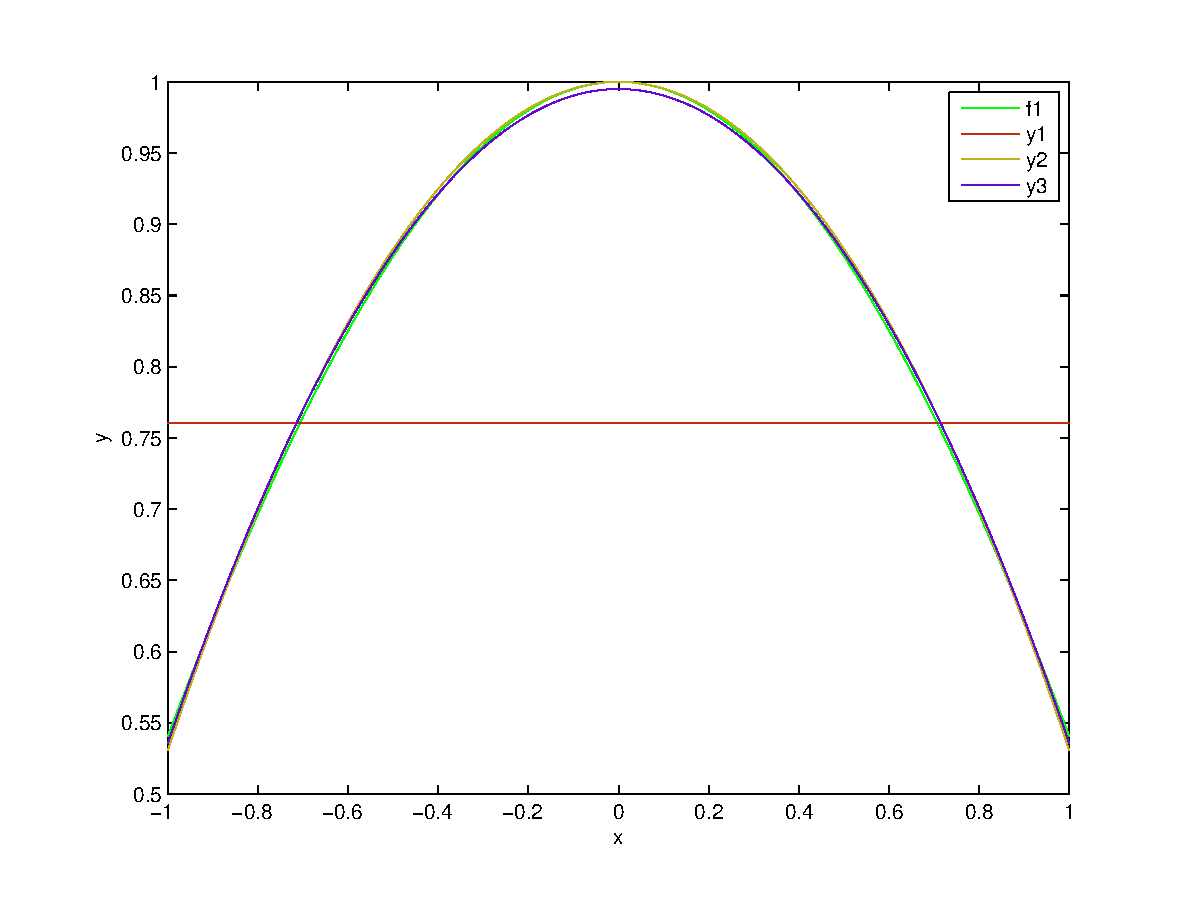
\includegraphics[width=\textwidth]{Jona/cheby_cos_interpolation.eps}
        \caption{Interpolerende Chebyshev veeltermen $y_{1},y_{2}$ en $y_{3}$ van respectievelijk graad $n=1,\dots,3$}
    \label{fig:cheb_cos_interpol}
    \end{subfigure}
    \begin{subfigure}[t]{0.45\textwidth}
        \centering
        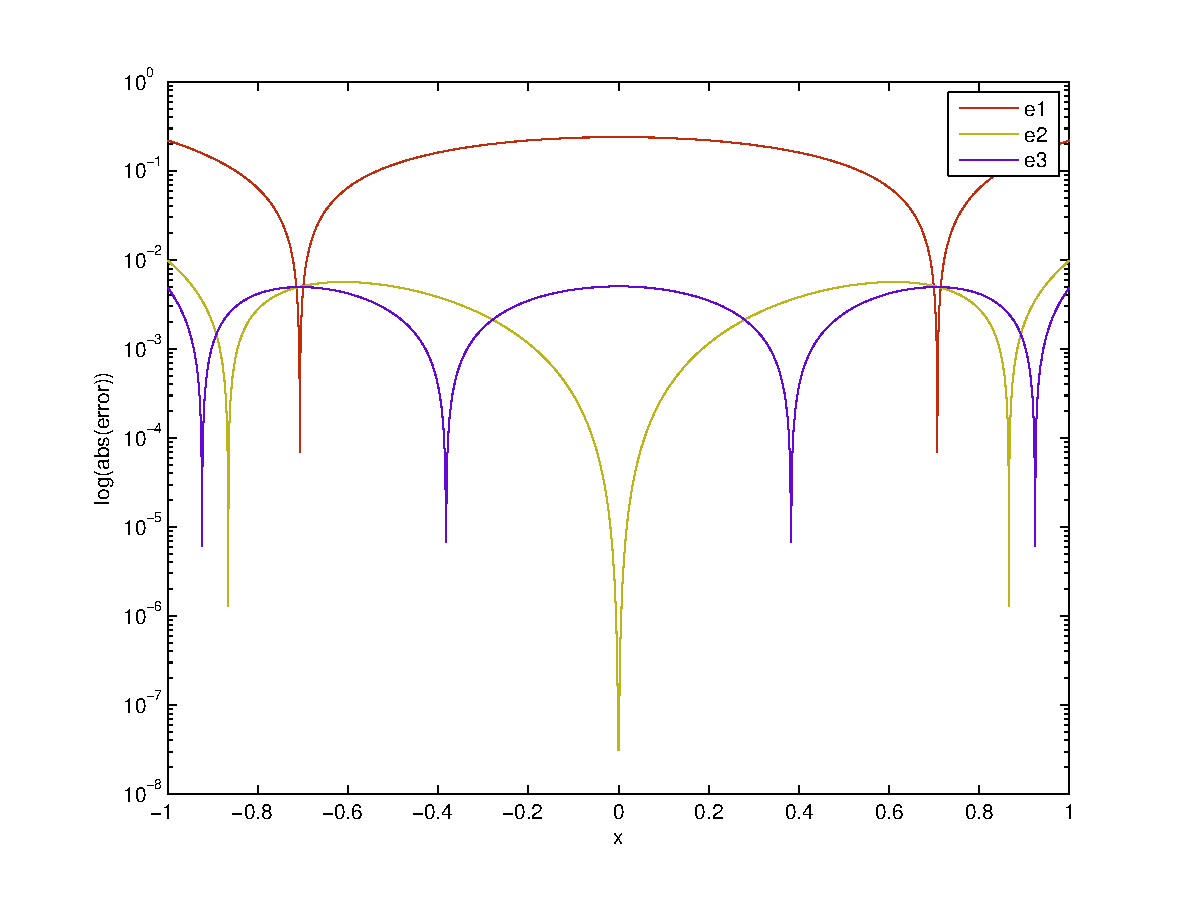
\includegraphics[width=\textwidth]{Jona/cheby_cos_error.eps}
        \caption{De fout $e_{n} = |y_{n}(t)-f(t)|$ van interpolerende Chebyshev veeltermen $y_{1},y_{2}$ en $y_{3}$ van respectievelijk graad $n=1,\dots,3$}
        \label{fig:cheb_cos_error}
    \end{subfigure}
    \caption{De functie $f_{1}(t) = cos(t)$ wordt benaderd in de nulpunten van de Chebyshev-veelterm van graad $n+1$ door middel van Chebyshev veeltermen}\label{fig:cheb_cos}.
\end{figure}

\begin{figure}
    \centering
    \begin{subfigure}[t]{\textwidth}
        \centering
        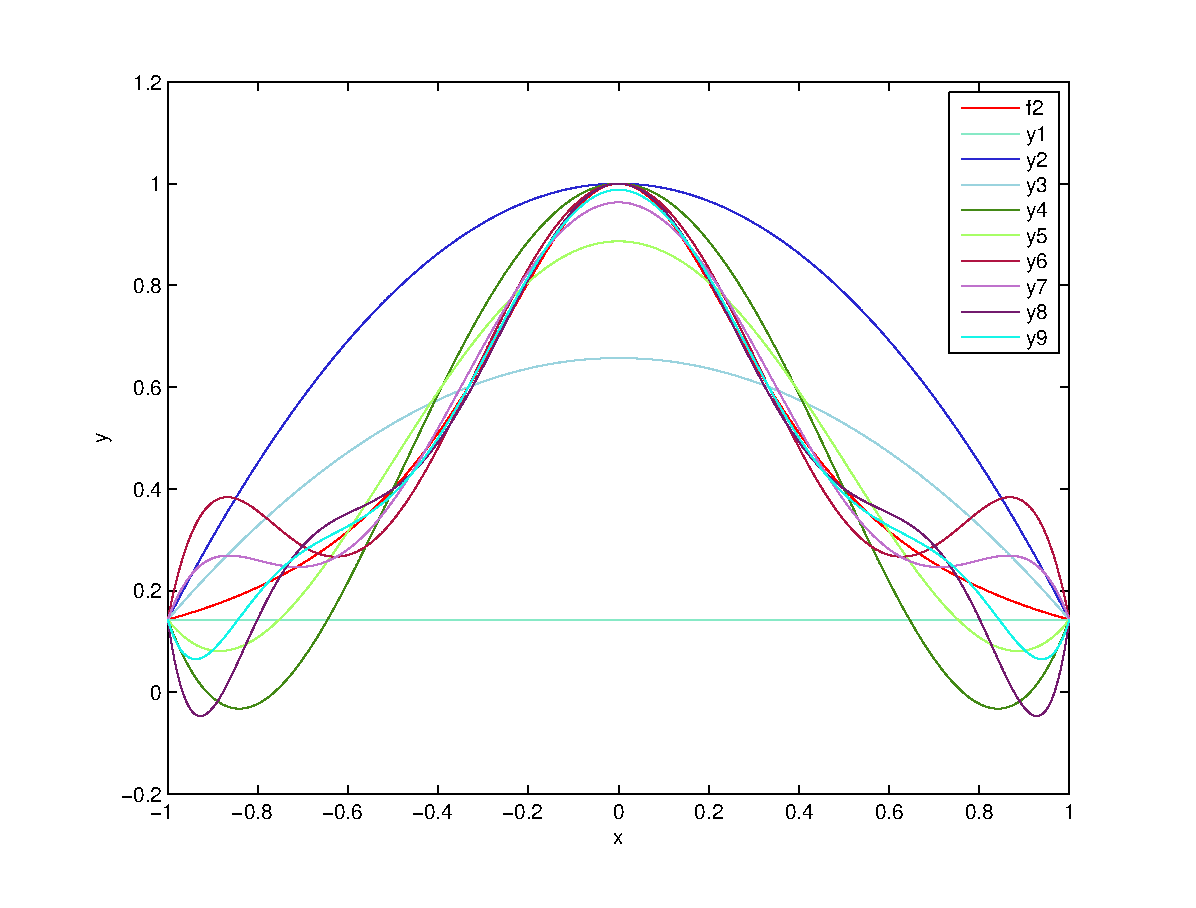
\includegraphics[width=\textwidth]{Jona/linspace_f2_interpolation.eps}
        \caption{Interpolerende Chebyshev veeltermen $y_{1},\dots,y_{9}$ van respectievelijk graad $n=1,\dots,9$}
        \label{fig:lin_f2_interpol}
        %\vspace*{1cm}
    \end{subfigure}
    \begin{subfigure}[t]{\textwidth}
        \centering
        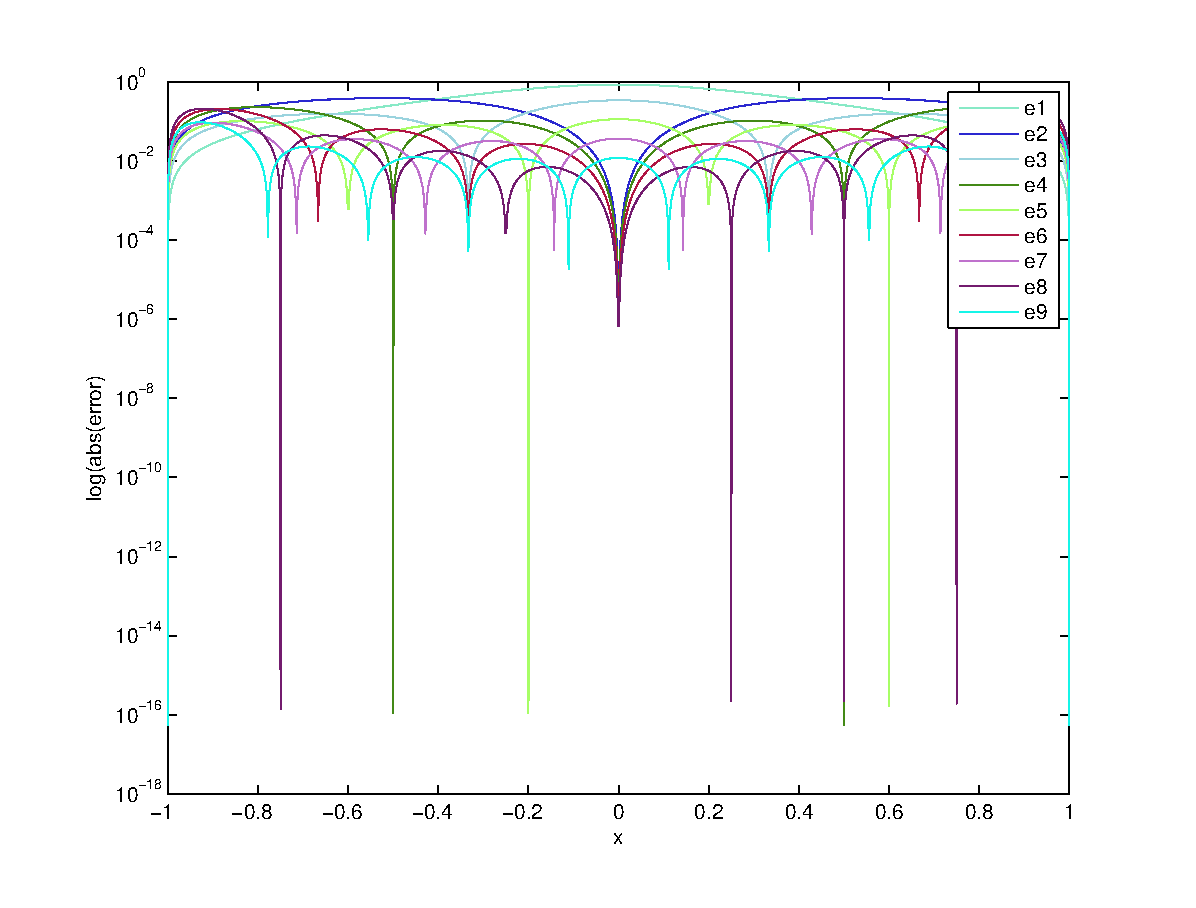
\includegraphics[width=\textwidth]{Jona/linspace_f2_error.eps}
        \caption{De fout $e_{n} = |y_{n}(t)-f(t)|$ van interpolerende Chebyshev veeltermen $y_{1},\dots,y_{9}$ van respectievelijk graad $n=1,\dots,9$}
        \label{fig:lin_f2_error}
        %\vspace*{1cm}
    \end{subfigure}
    \hfill
    \caption{De functie $f_{2}(t) = \frac{1}{1+6x^{2}}$ wordt benaderd in equidistant verdeelde interpolatiepunten door middel van Chebyshev veeltermen}\label{fig:lin_f2}.
\end{figure}

\begin{figure}
    \centering
    \begin{subfigure}[t]{\textwidth}
        \centering
        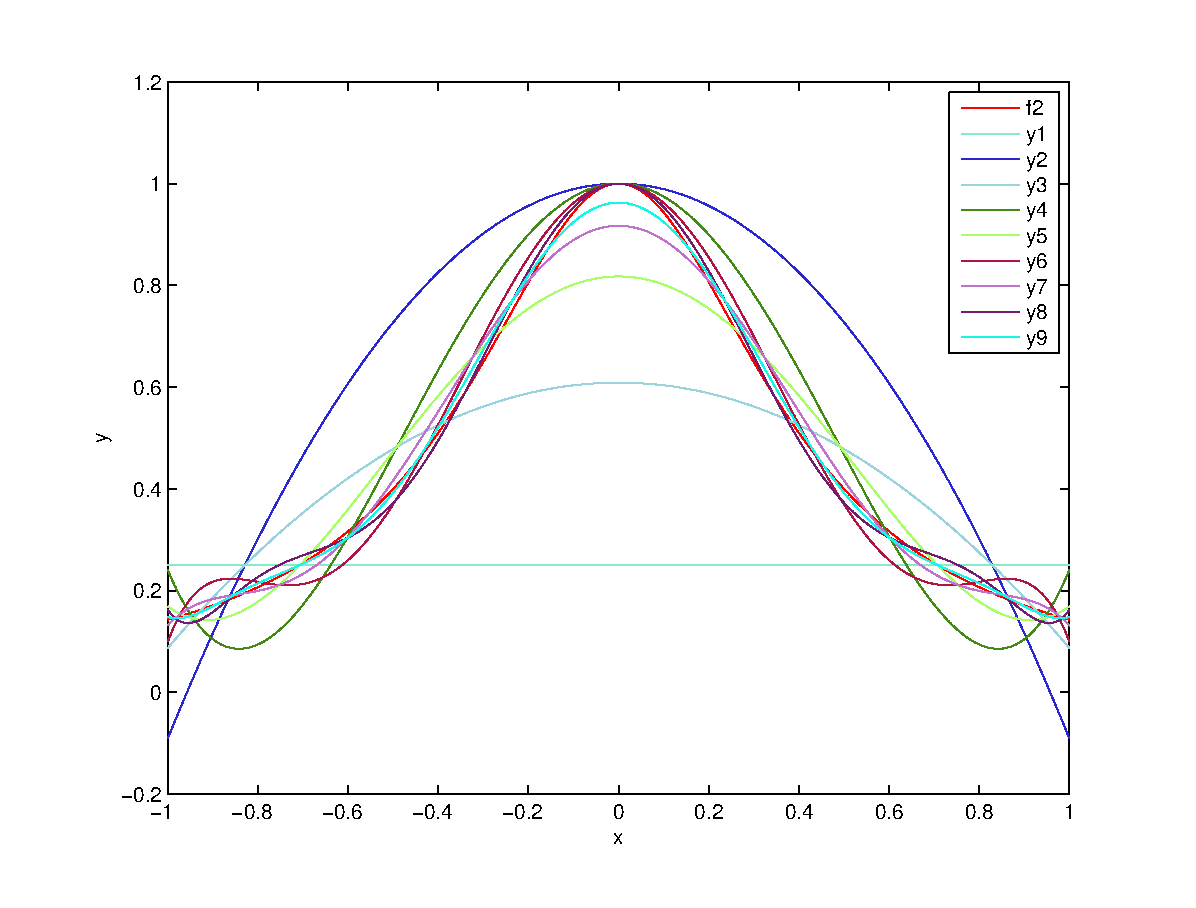
\includegraphics[width=\textwidth]{Jona/cheby_f2_interpolation.eps}
        \caption{Interpolerende Chebyshev veeltermen $y_{1},\dots,y_{9}$ van respectievelijk graad $n=1,\dots,9$}
        \label{fig:cheb_f2_interpol}
        %\vspace*{1cm}
    \end{subfigure}
    \begin{subfigure}[t]{\textwidth}
        \centering
        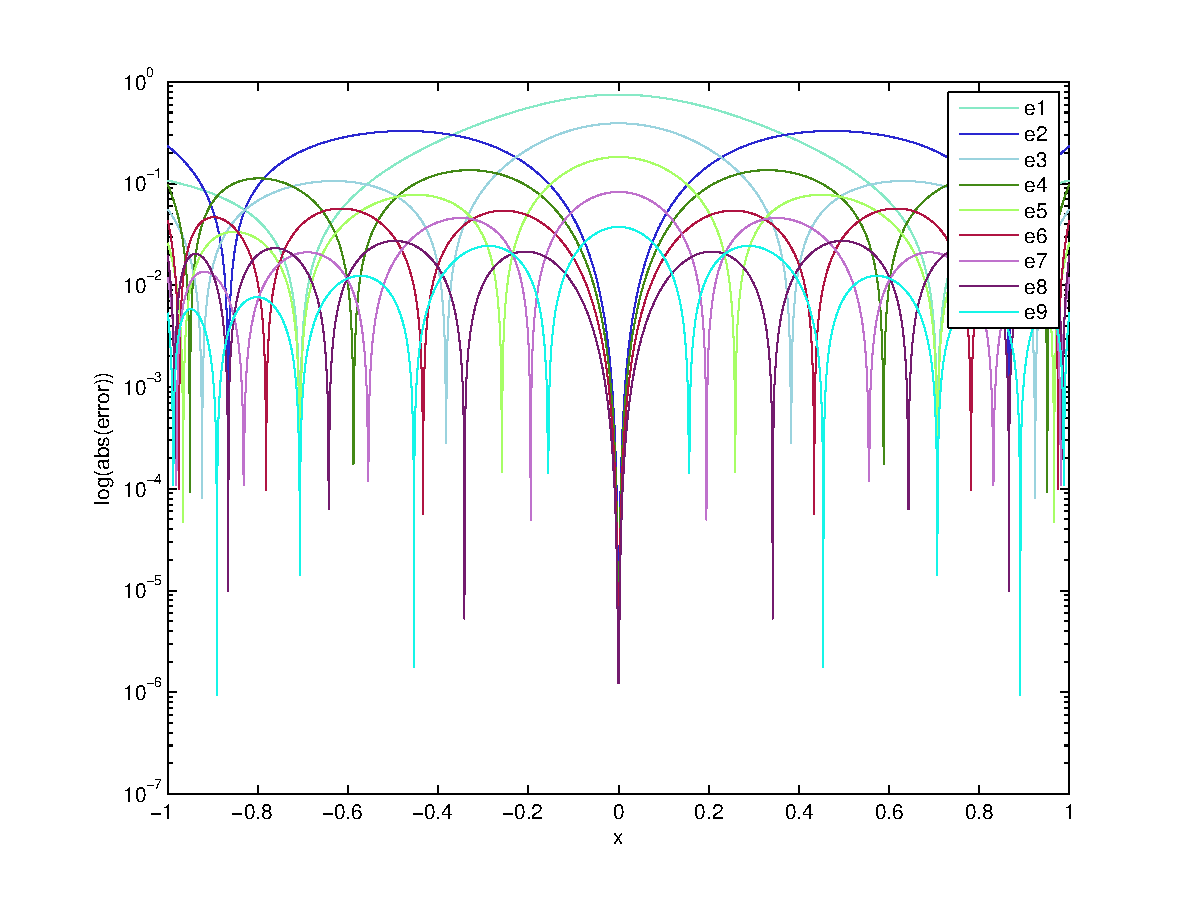
\includegraphics[width=\textwidth]{Jona/cheby_f2_error.eps}
        \caption{De fout $e_{n} = |y_{n}(t)-f(t)|$ van interpolerende Chebyshev veeltermen $y_{1},\dots,y_{9}$ van respectievelijk graad $n=1,\dots,9$}
        \label{fig:cheb_f2_error}
        %\vspace*{1cm}
    \end{subfigure}
    \hfill
    \caption{De functie $f_{2}(t) = \frac{1}{1+6x^{2}}$ wordt benaderd in in de nulpunten van de Chebyshev-veelterm van graad $n+1$ door middel van Chebyshev veeltermen}\label{fig:cheb_f2}.
\end{figure}

\begin{figure}
    \centering
    \begin{subfigure}[t]{0.45\textwidth}
        \centering
        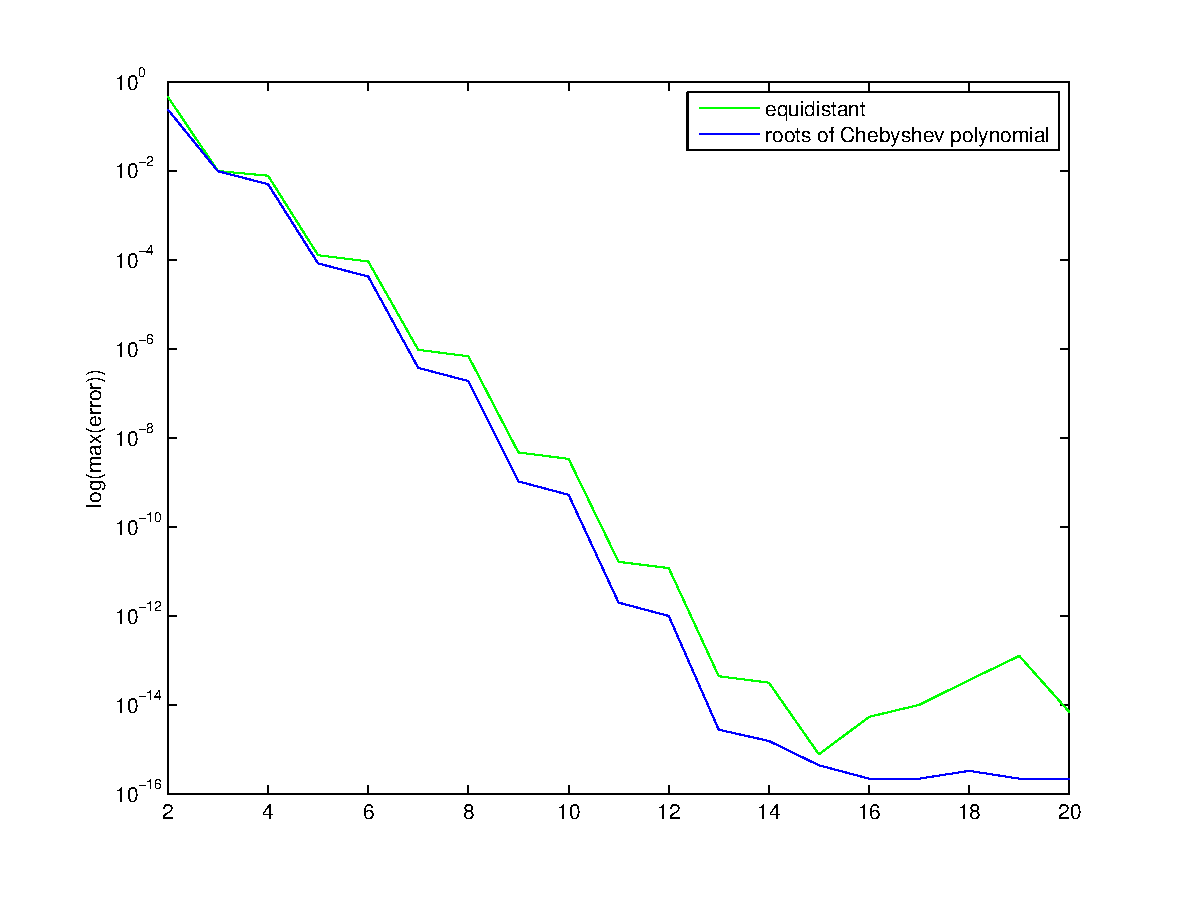
\includegraphics[width=\textwidth]{Jona/error_global_cos.eps}
        \caption{maximale fout $|y_{n}(t)-f(t)|$ in functie van stijgende graad $n$ voor equidistant verdeelde punten en nulpunten van de Chebyshev-veelterm van graad $n+1$}
        \label{fig:error_global_cos}
        %\vspace*{1cm}
    \end{subfigure}
    \begin{subfigure}[t]{0.45\textwidth}
        \centering
        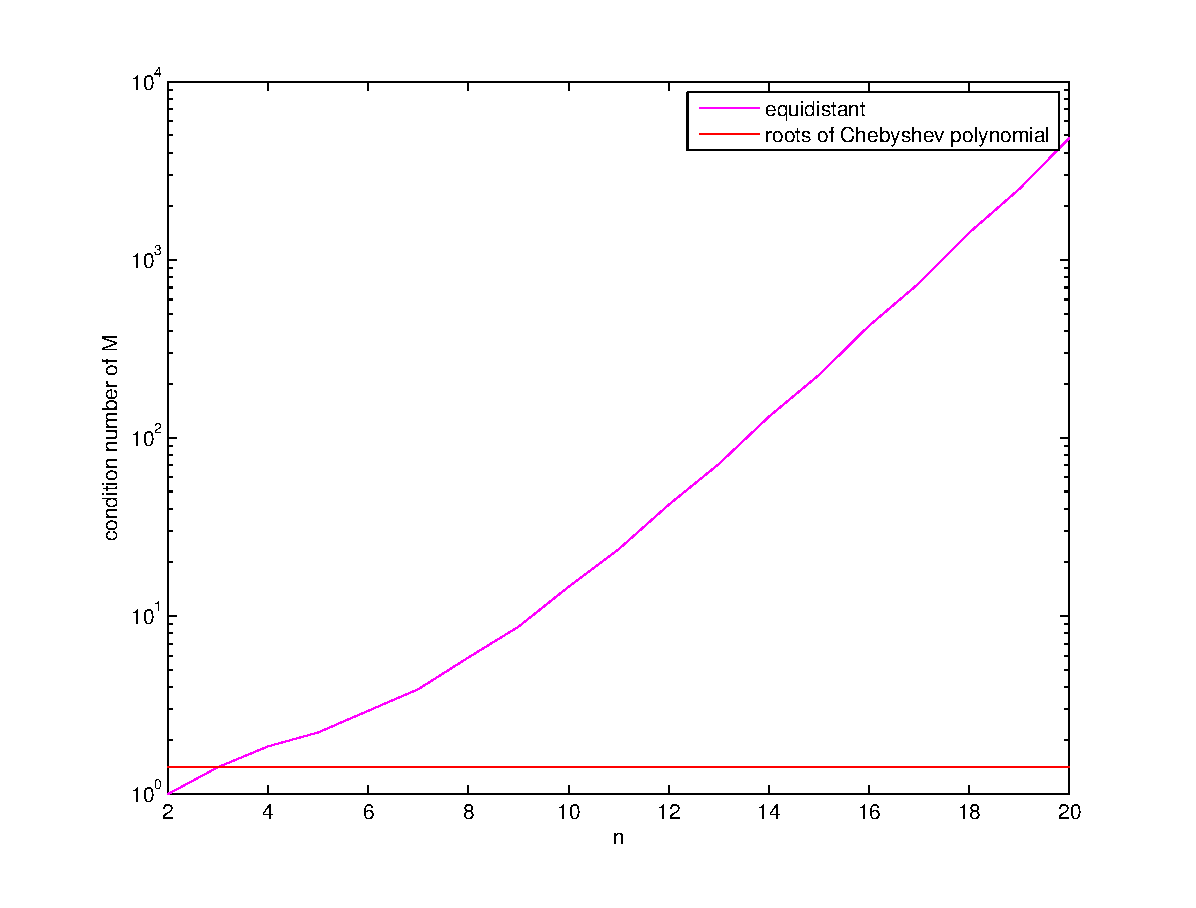
\includegraphics[width=\textwidth]{Jona/condition_cos.eps}
        \caption{conditiegetal $\kappa$ van de matrix $M$ in functie van stijgende graad $n$ voor equidistant verdeelde punten en nulpunten van de Chebyshev-veelterm van graad $n+1$}
        \label{fig:condition_cos}
        %\vspace*{1cm}
    \end{subfigure}
    \hfill
    \caption{Karakteristieken van de interpolerende veelterm van $f_{1}(t) = cos(t)$ in functie van de graad $n$}
    \label{fig:characteristics_cos}
    \end{figure}
    
\begin{figure}
    \centering
    \begin{subfigure}[b]{0.45\textwidth}
        \centering
        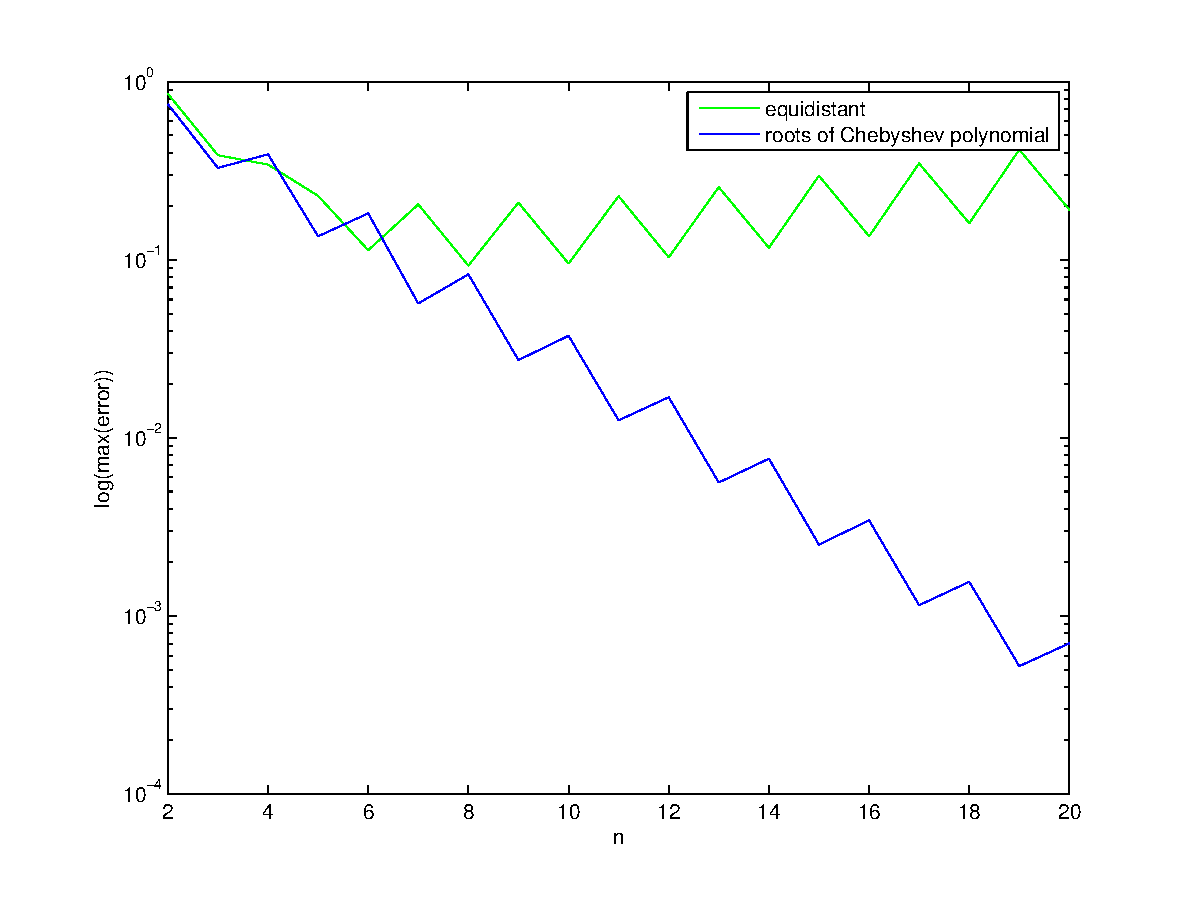
\includegraphics[width=\textwidth]{Jona/error_global_f2.eps}
        \caption{maximale fout $|y_{n}(t)-f(t)|$ in functie van stijgende graad $n$ voor equidistant verdeelde punten en nulpunten van de Chebyshev-veelterm van graad $n+1$}
        \label{fig:error_global_f2}
        %\vspace*{1cm}
    \end{subfigure}
    \begin{subfigure}[b]{0.45\textwidth}
        \centering
        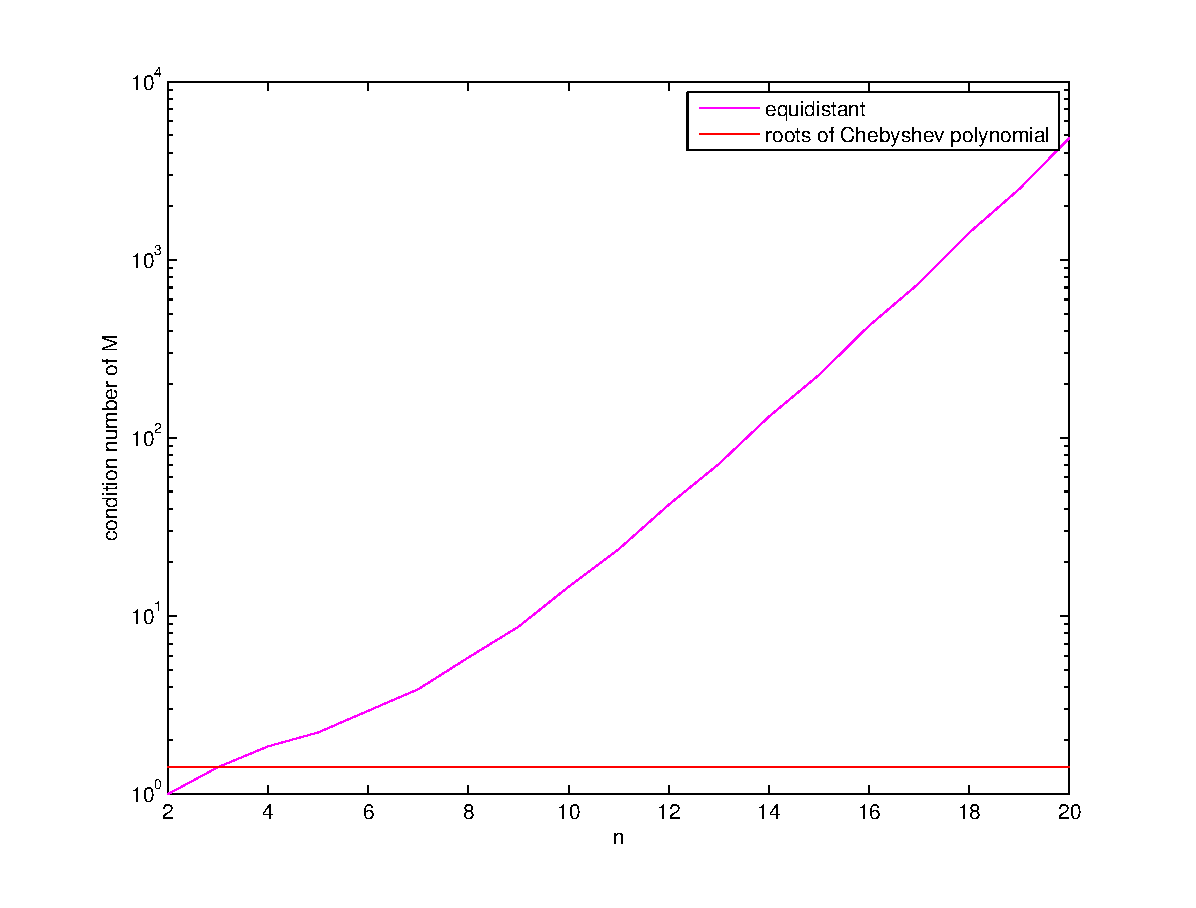
\includegraphics[width=\textwidth]{Jona/condition_f2.eps}
        \caption{conditiegetal $\kappa$ van de matrix $M$ in functie van stijgende graad $n$ voor equidistant verdeelde punten en nulpunten van de Chebyshev-veelterm van graad $n+1$}
        \label{fig:condition_f2}
        %\vspace*{1cm}
    \end{subfigure}
    \hfill
    \caption{Karakteristieken van de interpolerende veelterm van $f_{2}(t) = \frac{1}{1+6x^{2}}$ in functie van de graad $n$}
    \label{characteristics_f2}
    \end{figure}    
\opgave{5}
Het conditiegetal $\kappa$ van de matrix M wordt voorgesteld in figuur \ref{fig:condition_cos} en figuur \ref{fig:condition_f2}. De matrix horende bij de benadering van $f_{1}$ en $f_{2}$ heeft nagenoeg hetzelfde conditiegetal. Het conditiegetal stijgt bij gebruik van equidistante interpolatiepunten omdat de functiewaarden van de basis Chebyshev veeltermen dichter bij elkaar komen te liggen bij een stijgend aantal interpolatiepunten. Hierdoor worden de kolommen van $M$ meer en meer afhankelijk. Dit resulteert in een stijgend conditiegetal. Door de nulpunten van de Chebyshev veelterm te nemen blijft het conditiegetal klein en constant.

Een groot conditiegetal betekent dat het resultaat van een kleine perturbatie op de elementen van $M$ sterk afwijkt van het oorspronkelijk resultaat. De co\"effici\"enten $c_{i}$ zullen dus sterk veranderen bij een kleine wijziging op de interpolatiepunten. Hierdoor zal de veelterm in de intervallen rond de interpolatiepunten wijzigen. In de interpolatiepunten zal de wijziging ongeveer gelijk zijn aan de perturbatie aangezien de interpolatievoorwaarde($y_{n}(x_{i}) = f(x_{i})$)nog steeds voldaan moet worden.

Als we aannemen dat het stelsel in \textsc{Matlab} achterwaarts stabiel wordt opgelost, dan hangt de nauwkeurigheid van de interpolerende veelterm af van het conditiegetal. Dit wordt uiteengezet in \textbf{Theorem 15.1 Trefethen and Bau}. Als het conditiegetal stijgt, dan zal de nauwkeurigheid zakken en dus de fout op de co\"effici\"enten vergroten. Dit betekent niet noodzakelijk dat ook de nauwkeurigheid van interpolerende veelterm zal verminderen. In figuur \ref{fig:characteristics_cos} stijgt het conditiegetal ook voor equidistant verdeelde interpolatiepunten maar toch neemt de fout ook nog af. In figuur \ref{characteristics_f2} neemt de nauwkeurigheid van de interpolerende veelterm wel af. 
\opgave{6}
De opbouw van het algoritme is als volgt:
\paragraph*{}
Eerst wordt het aantal rijen $N$ gezocht van de matrix x om vervolgens de $N$-punts FFT uit te voeren.Vervolgens worden de co\"{e}ffici\"{e}nten $X_{K+1}, \dots ,X_{\frac{N}{2}}$ gelijk aan nul gesteld. In diezelfde operatie worden ook meteen de corresponderende $X_{N-k}$ co\"{e}ffici\"{e}nten gelijk aan nul gesteld vanwege de symmetrie. Om de oorspronkelijke functie te kunnen evalueren in een aantal punten $M \geq N$, worden de volgende relaties gebruikt:
\begin{equation}
    \centering
        \begin{cases}
            Y_k=\frac{M}{N}X_k & k=0,\dots,\frac{N}{2}-1 \\
            Y_k=\frac{M}{N}\frac{X_k}{2} & k=\frac{N}{2} \\
            Y_k=0 & k=\frac{N}{2}+1,\dots,\frac{M}{2}
        \end{cases}
\end{equation}
Tenslotte kan via de $M$-punts inverse FFT de benadering voor het oorspronkelijke signaal gevonden worden.
\paragraph*{}
De \textsc{Matlab}-code bevindt zich in bijlage 4.
\opgave{7}
Wanneer alleen de K eerste $X_k$ co\"{e}ffici\"{e}nten behouden worden, worden de hogere frequenties uit het signaal weggehaald. Dit komt overeen met een laagdoorlaatfiltering van het signaal. Er gaat enkel informatie verloren als er wel degelijk frequenties aanwezig zijn in het oorspronkelijke signaal die co\"{e}ffici\"{e}nten $X_{K+1}, \dots ,X_{\frac{N}{2}}$ verschillend van nul veroorzaken.

Als voorbeeld beschouwen we een signaal in functie van de tijdsparameter $t$ samengesteld uit 10 verschillende frequenties
\begin{align}
c=\sum_{k=1}^{10} \sin{2\pi kt}
\end{align}
Wanneer dit signaal in 512 punten gesampled wordt en er daarna de FFT van genomen wordt, bekomt men Figuur \ref{fig:periotriga}. Hetzelfde resultaat wordt bekomen door $K=256$ te nemen. Noteer dat de FFT er voor zorgt dat er ook schijnbaar frequenties aanwezig zijn bij $11,12,\dots$. De waarden verschillend van nul bij deze frequenties ontstaan door de keuze van het venster en worden in de verdere behandeling verwaarloosd.

Als $K=10$ wordt genomen, worden er geen nuttige frequenties verwijderd uit het signaal en bijgevolg is het benaderende signaal exact gelijk aan het oorspronkelijke signaal zoals te zien is in Figuur \ref{fig:periotrigb}.

De laagdoorlaatfiltering wordt pas echt duidelijk wanneer $K=5$ wordt gesteld. Als gevolg van deze keuze van $K$ verdwijnt de helft van de frequenties in de benadering zoals te zien in de rechterfiguur van Figuur \ref{fig:periotrigc}. Aangezien de hogere frequenties eenvoudigweg op nul gezet worden, verdwijnt ook de energie die in deze frequenties vervat zit wat resulteert in een signaal met een minder grote amplitude. Ook in de linkerfiguur van Figuur \ref{fig:periotrigc} is te zien dat er een veel \textit{geleidelijker} verloop is van de veelterm.
\begin{figure}
    \centering
    \begin{subfigure}[b]{\textwidth}
        \centering
        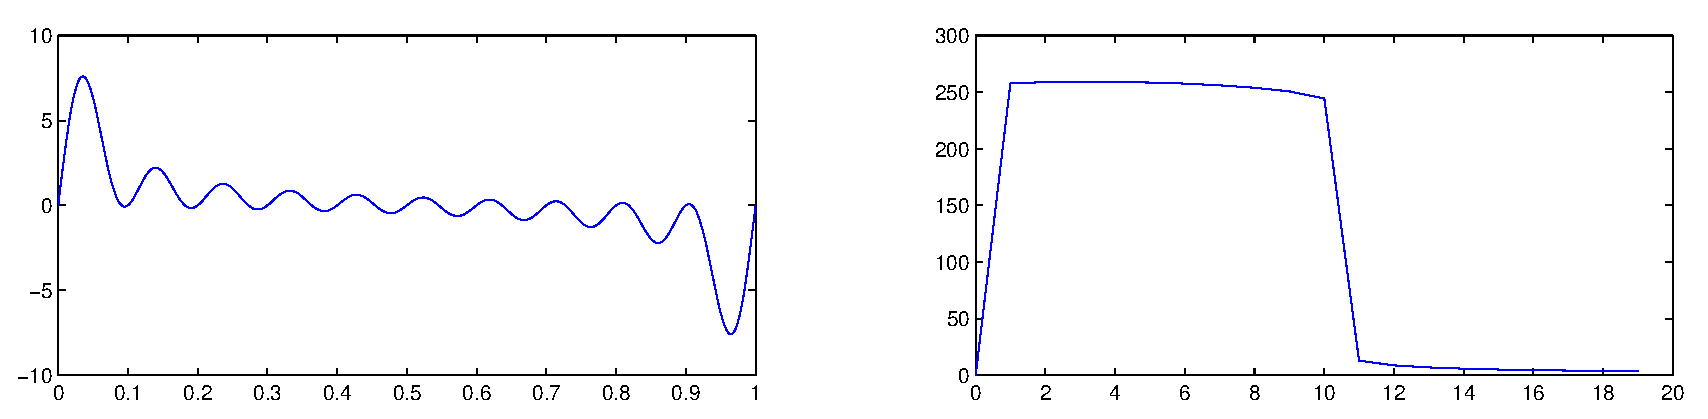
\includegraphics[width=\textwidth, height=0.3\textwidth]{periotriga.eps}
        \caption{Oorspronkelijke functie met $K=256$}
        \label{fig:periotriga}
        \vspace*{1cm}
    \end{subfigure}
    \begin{subfigure}[b]{\textwidth}
        \centering
        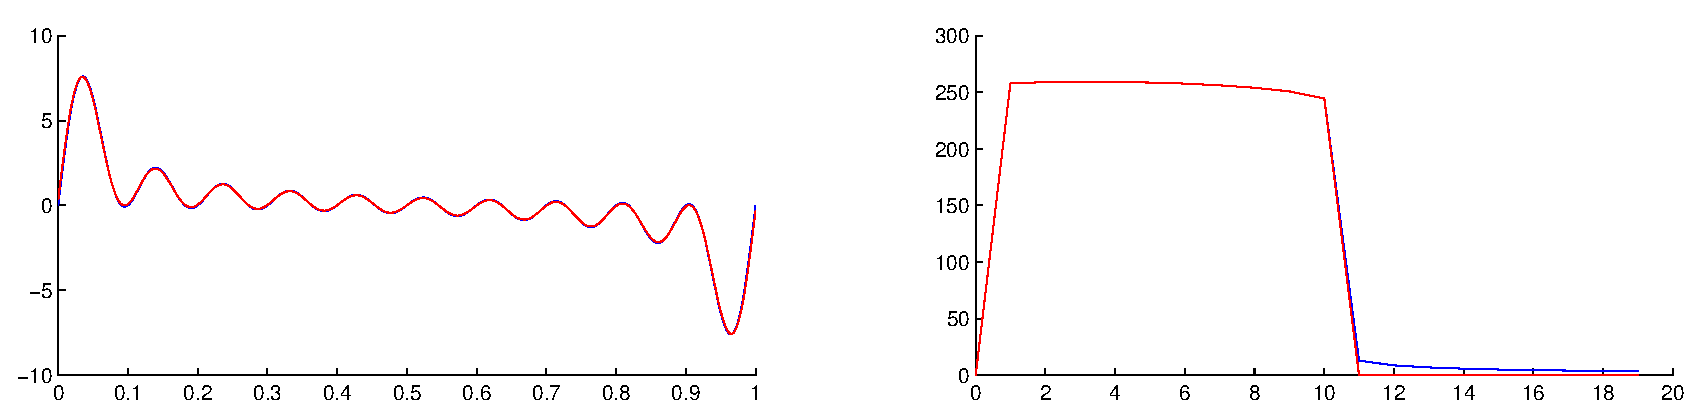
\includegraphics[width=\textwidth]{periotrigb.eps}
        \caption{Benaderende functie met $K=10$}
        \label{fig:periotrigb}
        \vspace*{1cm}
    \end{subfigure}
    \hfill
    \begin{subfigure}[b]{\textwidth}
        \centering
        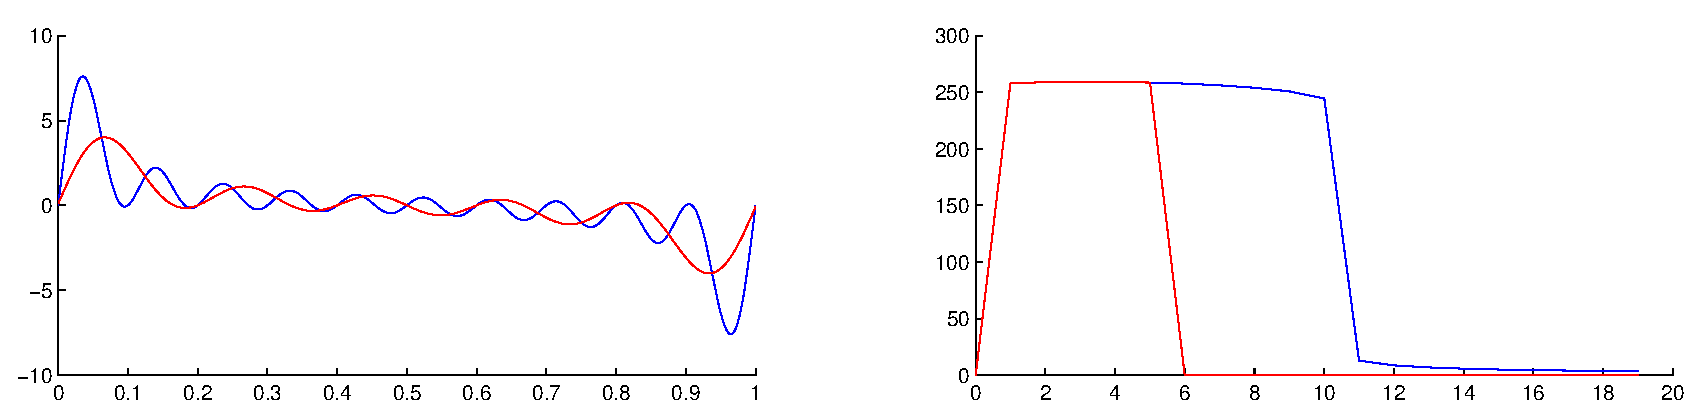
\includegraphics[width=\textwidth]{periotrigc.eps}
        \caption{Benaderende functie met $K=5$}
        \label{fig:periotrigc}
        \vspace*{1cm}
    \end{subfigure}
    \caption{Illustratie van de invloed van de parameter $K$ op de benadering (rood) van een periodieke functie (blauw) met aan de linkerkant de veelterm en aan de rechterkant de FFT van deze veelterm weergegeven over een nuttig domein. ($M = N = 512$)}\label{fig:periotrig}.
\end{figure}
\opgave{8}
In Figuur \ref{fig:periotrigclick} wordt een benadering geconstrueerd voor het $\infty$ teken aan de hand van de functies \textit{click()} en \textit{periotrig(x,K,M)}. In de linkse deelfiguur zijn de oorspronkelijke punten weergegeven die met \textit{click()} zijn getekend. De rechterfiguur toont een periodieke interpolerende en benaderende trigonometrische veelterm voor deze punten.

Aangezien het teken $\infty$ geschreven kan worden als een speciaal geval (met name \textit{het lemniscaat van Gerono}) van de meer algemene \textit{Lissajousfiguur}, is deze benadering uiterst geschikt omdat de parametrisaties bij een \textit{Lissajousfiguur} van de volgende vorm zijn:
\begin{equation}
    \centering
        \begin{cases}
            x=\sin (\alpha t+\delta)\\
            y=\sin (\beta t)
        \end{cases}
\end{equation}
Wanneer in deze vergelijkingen de waarden $\alpha=1$,$\beta=2\alpha=2$ en $\delta=0$ worden genomen, verkrijgt men Figuur \ref{fig:lissajous}.
\begin{figure}
    \centering
    \begin{subfigure}[b]{0.4\textwidth}
        \centering
        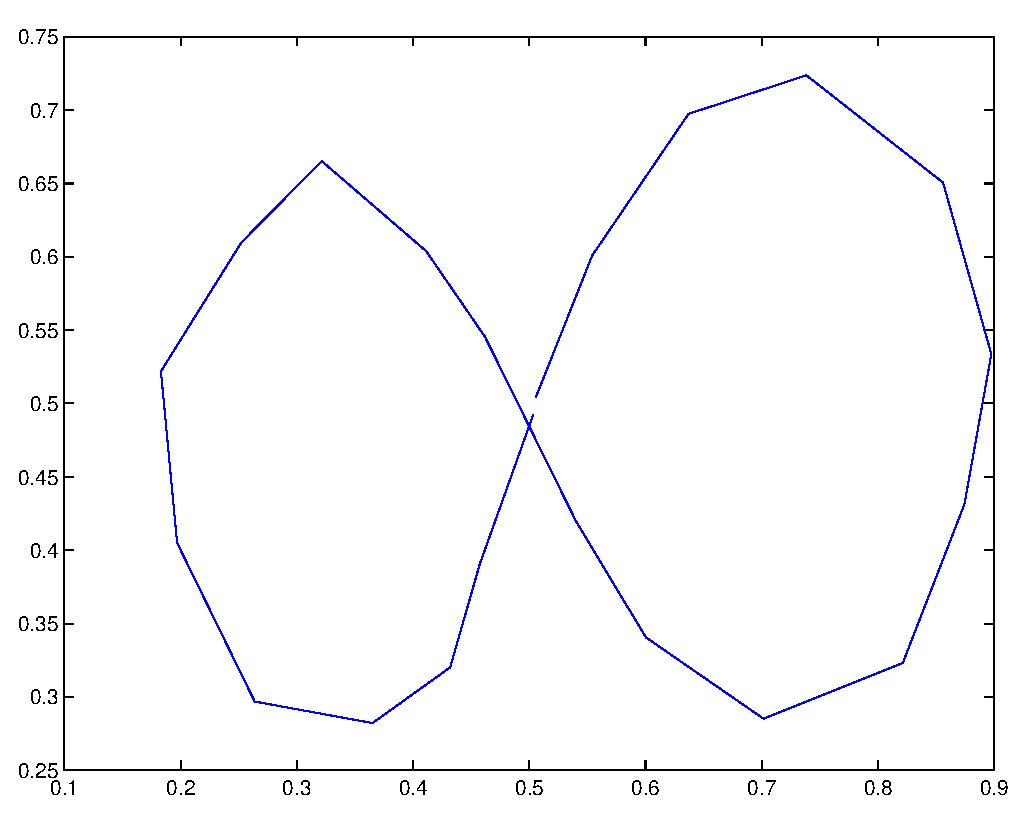
\includegraphics[width=\textwidth]{infclick.eps}
        \caption{Punten met \textit{click()}}
        \label{fig:periotriga}
    \end{subfigure}
    \begin{subfigure}[b]{0.4\textwidth}
        \centering
        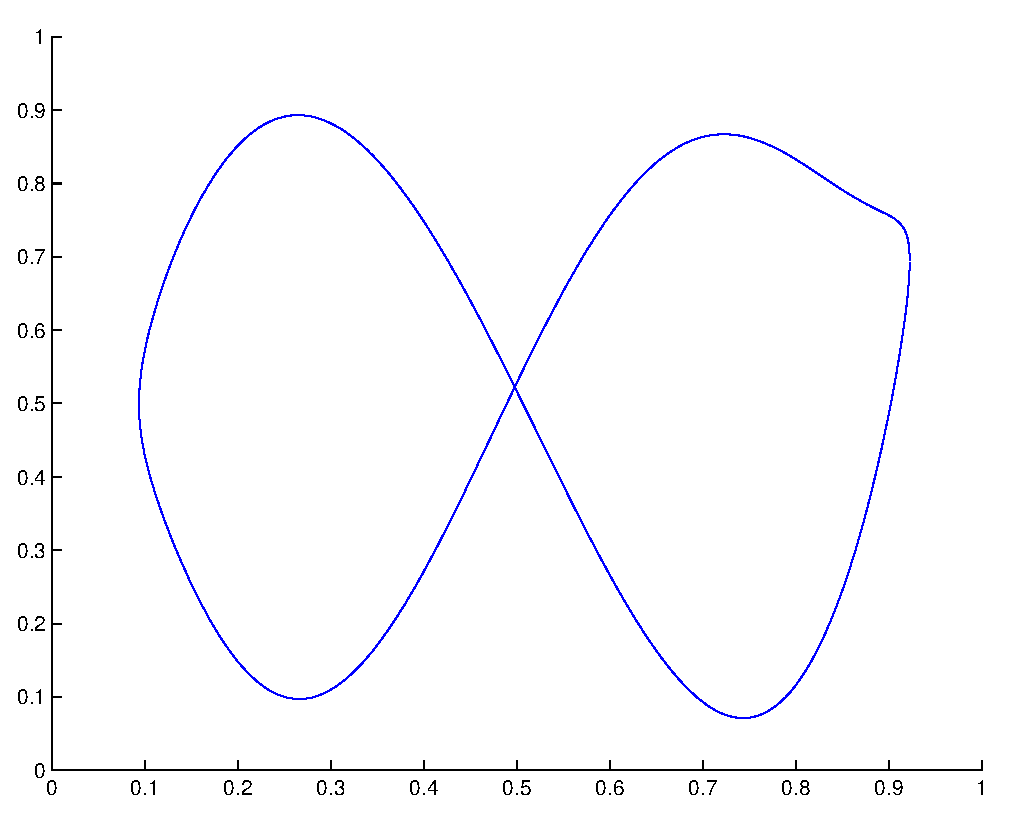
\includegraphics[width=\textwidth]{inftrig.eps}
        \caption{Benaderende functie}
        \label{fig:periotrigb}
    \end{subfigure}
    \hfill
    \caption{$\infty$ teken benaderd}\label{fig:periotrigclick}.
\end{figure}
\begin{figure}
        \centering
        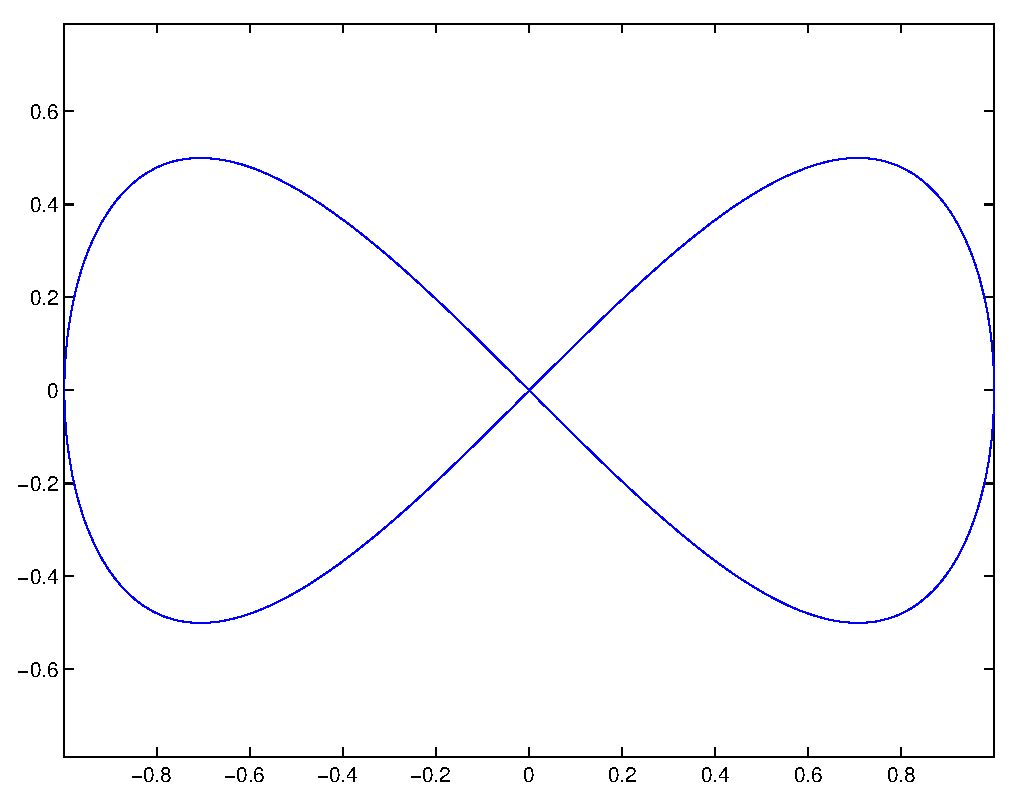
\includegraphics[width=0.85\textwidth]{lissajous.eps}
        \caption{Het $\infty$ teken onder de vorm van een Lissajousfiguur}
        \label{fig:lissajous}
    \end{figure}
\newpage
\section*{Bijlage 1} 
\lstinputlisting{Jona/poly_zeros.m}
\label{bijlage:1}
\section*{Bijlage 2} 
\lstinputlisting{Jona/eval_recursion.m}
\label{bijlage:2}
\newpage
\section*{Bijlage 3} 
\lstinputlisting{Jona/interpolate.m}
\label{bijlage:3}
\newpage
\section*{Bijlage 4} 
\lstinputlisting{periotrig.m}
\label{bijlage:4}
\end{document}